\versoquote{Но природа не справляется с логикой, с нашей человечес- кою логикой: у ней есть своя, которую мы не понимаем и не признаем до тех пор, пока она нас, как колесом, не переедет.}{Иван Сергеевич Тургенев}
%Nature cares nothing for logic, our human logic: she has her own, which we do not recognize and do not acknowledge until we are crushed under its wheel. --Ivan Turgenev
\chapter{Junction Models}\label{ch:junctions}
\loftchap{Junction Models}
\chapterprecis{Methodology used to construct high precision Josephson junction models of varying stoichiometry and density.}

\thought{The jury is still out} when it comes to the specific location of strongly coupled TLSs inside Josephson junctions, and as we've seen in \cref{sec:micromod}, many perchance competing microscopic models exist that attempt to describe their origin.
One possible way of distinguishing between these options (including the one posited in \cref{sec:conjecture}) is to develop complete atomistic models of the Josephson junction and study the many spatial configurations of the amorphous tunneling barrier.

From a quantum simulation point of view, this is not a trivial problem.
Crystalline symmetries usually invoked to minimise calculations cannot be used to reduce the state space of the oxide barrier of a junction due to its amorphous nature.
However, forming such atomistic models using molecular mechanics and \textit{ab initio} methods is the focus of this chapter.

Initially, we discuss the computational complexities of simulating oxide formation directly in \cref{sec:simjjform}, followed by the specific methods that have been implemented in \cref{sec:jjmodel}.
\Crefrange{sec:gr}{sec:coord} examine a number of techniques which assist in validating the resultant models in terms of expected configurational properties and experimental data.
Finally a summary in \cref{sec:jjsum} which outlines some technical uses for these models outside the main scope of this thesis.

\section{Simulating the Junction Formation Process}\label{sec:simjjform}

Josephson junctions may be constructed from any superconducting material with any insulating or non-superconducting metal barrier to invoke a weak link coupling.
A popular material choice involves the use of aluminium as the superconducting material, and an amorphous oxide layer as an insulating barrier.
\Cref{sec:formation} discusses the shadow evaporation techniques usually undertaken to grow a $\sim2$ nm amorphous layer which may vary in stoichiometry, density and thickness.

Simulating oxide layer growth is in general a difficult problem as the time scale of the oxide growth ($\sim\,$minutes) is orders of magnitude greater than typically achievable molecular dynamics timescales (ps--ns).
One standard approach is to perform the simulation at elevated temperatures and gas pressures ($\ge 1$ atm)~\cite{Campbell1999, Zhou2005, Hasnaoui2005}.
This accelerates the oxidation process, making the computation feasible on current high performance computing infrastructure.
However, it also removes the simulation from the reality of experimental junction formation, where pressures range between $10^{-9}$ and $10^{-3}$ atm~\cite{Morohashi1987, Kohlstedt1993, Jeurgens2002}.
It remains to be seen whether any fundamental physics is neglected by adopting this approximation.

An alternative approach is to form an amorphous layer via direct melt and quench~\cite{Vashishta2008,Sheng2012}.
This method has the advantage of computational simplicity and speed, however the resulting layers are not necessarily representative of the true physical situation and therefore benchmarking against other methods and experiment is critical.
Generating stoichiometry or density gradients across an artificial junction is not something that can be simulated directly using this process, so to investigate the effect of these properties, a number of constant density and stoichiometry models were produced. A more sophisticated method, closely mimicking the oxygen deposition process and examining the effects of layer thickness is the subject of M. Cyster's PhD dissertation.

\section{Model Construction}\label{sec:jjmodel}

To obtain realistic, high precision atomic positions, computational models of the junction were created using a combination of molecular mechanics and DFT.
A $4\!\times\!4\!\times\!5$ supercell of bulk aluminium (measuring $16.168\times16.168\times20.183$ \AA) representing both the top and bottom slabs was relaxed in the DFT code \sw{VASP}~\cite{Kresse1994, Kresse1996, Kresse1996a} using a projector-augmented wave (PAW) potential~\cite{Kresse1999, Blochl1994}.
Exchange-correlation interactions were evaluated using the PBE functional~\cite{Perdew1996}; a $7\!\times\!7\!\times\!7$ $\Gamma$ centered Monkhorst Pack K point mesh and a plane wave cutoff of $250$ eV.\nomdef{BA}{\AA}{Ångström, 1 \AA $= 10^{-10}$ m}

Formation of the amorphous \ce{AlO_x} layers required a number of preparation steps to accurately represent experimental results.
Corundum was used as a basis for all the constructed junction models as it represents the low temperature and pressure phase of aluminium oxide.
Experimental investigations of stoichiometry suggest, in general, an oxygen deficiency with oxide O/Al ratios varying between 0.6 and 1.4~\cite{Tan2005}, which are highly dependent on the fabrication process.
In response to this, we construct models with four stoichiometries: \ce{AlO_{0.8}}, \ce{AlO_{1.0}}, \ce{AlO_{1.25}} and \ce{AlO_{1.5}}.
The oxide density may also be an important formation variable.
For simplicity we identify oxide density as a fractional value of the (average) corundum density: $4.05$ g/cm$^\text{3}$, and construct junctions with 0.5, 0.625, 0.75, 0.875 \& 1.0 density fractions for each stoichiometry listed above.
A value of $3.2$ g/cm$^\text{3}$ is typical~\cite{Barbour1998} (which corresponds to a density fraction of 0.8).

Using \ce{AlO_{1.25}} with a density fraction of 0.75 as an example, a $6\!\times\!6\!\times\!1$ supercell of corundum was geometry optimised in the software package \sw{GULP}~\cite{Gale2003}, employing the empirical Streitz-Mintmire potential~\cite{Streitz1994} which can capture the variable oxygen charge states when present in a predominantly metallic environment. This capability is particularly important here, as a Josephson junction has two metal-oxide interfaces.
This large superstructure was required due to the trigonal nature of the lattice, as it was then cut down such that the $xy$ plane of the bulk aluminium slab could be covered.
A non-periodic slab of corundum measuring $16.168\!\times\!16.168\!\times\!11.982$ \AA\ was the result of this process.
Oxygen atoms were randomly removed from the corundum lattice until the appropriate stoichiometry of \ce{AlO_{1.25}} was obtained and the cell was shortened in the $z$-direction to achieve a 0.75 fractional multiple of the corundum density.
These changes add a lot of force onto the structure, so a geometry optimisation (in \sw{GULP}) was undertaken at this stage to minimise energy contributions.
To simulate the oxygen deposition phase and generate the amorphous nature of these layers, the structure was then annealed using NVT molecular dynamics at $3000$ K for $3$ µs and quenched to $350$ K over a $1.5$ µs period.

The \ce{AlO_{1.25}} layer was inserted between two bulk Al supercells described above with $0.5$ \AA\ of vacuum space on each side.
The junction was further annealed to simulate a metal--metal--oxide interface reconstruction using \sw{VASP} NVT Molecular Dynamics at $300$ K until equilibrium was reached (approximately $250$ ionic steps), then geometry optimised using a $2\!\times\!2\!\times\!1$ $\Gamma$ centered Monkhorst Pack K point mesh and a $450$ eV plane wave cutoff to obtain the final model, depicted in \cref{fig:povray}.

\begin{figure}[htp]
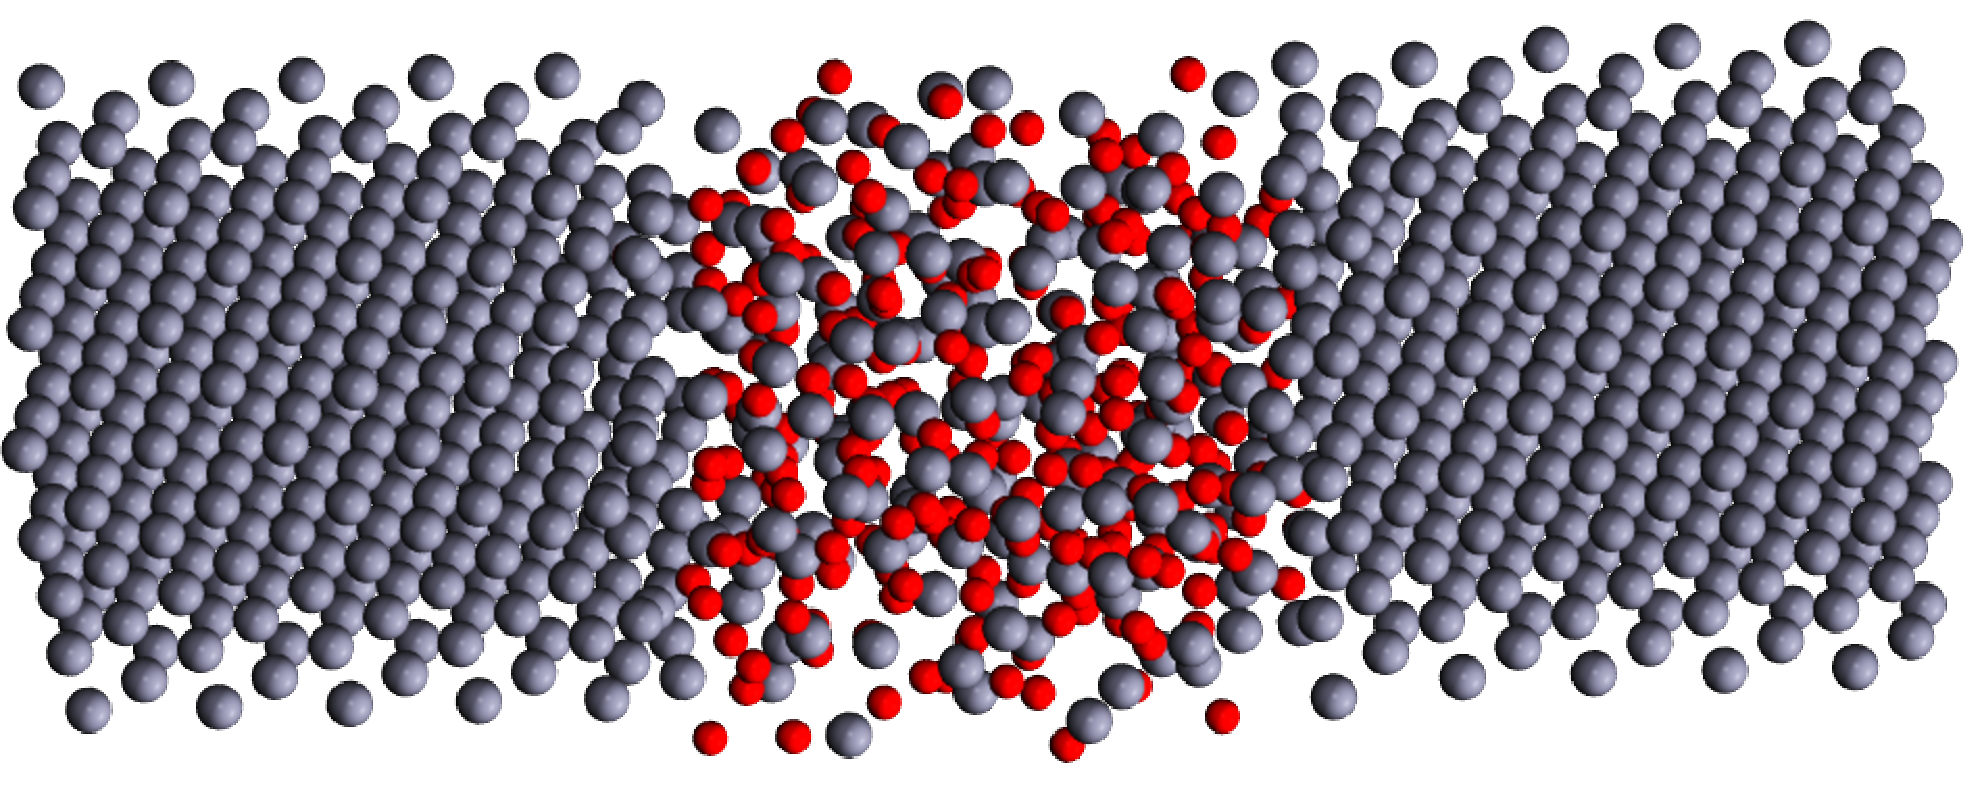
\includegraphics[width=0.9\textwidth]{figures/AlO125_075}
\caption[Atomistic Josephson Junction Model]{\label{fig:povray}Model of a Josephson junction comprised of aluminium \resizebox{!}{0.7em}{
\includegraphics{figures/jjal}} and oxygen \resizebox{!}{0.5em}{
\includegraphics{figures/jjo}}. Two superconducting regions composed only of aluminium, separated by an amorphous AlO$_{1.25}$ barrier with a density 0.75 times that of corundum.}%
\end{figure}

For comparison, junctions were also modelled without the added computational overhead of DFT by solely employing \sw{GULP} and the Streitz-Mintmire potential.
The construction process of these models matches the procedure above, but interchanges the \textit{ab initio} optimisations of the oxide layer with an empirical framework.

\section{Radial Distribution Function \texorpdfstring{$G(r)$}{G(r)}}\label{sec:gr}
To validate our models against experimental observations, we perform a number of statistical tests to scrutinize the structures.
First we must ensure that the oxide layer of the junctions are in fact amorphous in nature.
We employ a projected radial distribution function
\begin{equation}
G(r) = \lim_{dr \to 0}\frac{p(r)}{4\pi\left(N_{\mathrm{pairs}}/V\right)r^2dr}
\label{eq:gr}
\end{equation}
where $r$ is the distance between a pair of particles, $p(r)$ is the average number of atom pairs found at a distance between $r$ and $r + dr$, $V$ is the total volume of the system, and $N_{\mathrm{pairs}}$ is the number of unique pairs of atoms~\cite{Levine2011}.\nomdref{CN}{$N_{\mathrm{pairs}}$}{Number of unique atomic pairs in a radial distribution function}{eq:gr}\nomdref{CV}{$V$}{Total volume contained in a radial distribution function}{eq:gr}\nomdref{Cpr}{$p(r)$}{Average number of atom pairs found at a distance between $r$ and $r + dr$ in a radial distribution function}{eq:gr}\nomdref{Cgr}{$G(r)$}{Radial distribution function}{eq:gr}
This function was calculated for each stoichiometry and density configuration using oxygen as the reference species, and aluminium atoms in the amorphous region along with the superconducting bulk as the projection species. \Cref{fig:groptis} depicts the results of this analysis.

\begin{figure}[htp]
\resizebox{0.8\textwidth}{!}{\includestandalone{figures/groptis}}
\caption[Radial Distribution Function]{\label{fig:groptis}Evolution of the oxygen projected radial distribution function $G(r)$. Crystalline corundum \plotline{line width=1pt,color=gray!50}; Metal--oxide interface before \plotline{line width=1.5pt,dashdotted, color=Set1-5-3} and after \plotline{line width=1.5pt,dashed, color=Set1-5-2} reconstruction; final optimised geometry \plotline{line width=2pt,color=Set1-5-1}.}%
\end{figure}

A major peak is visible centered around $1.85$ \AA, which corresponds to contributions from the two Al--O bond distances, $1.852$ \AA\ and $1.971$ \AA\ of the corundum crystal~\cite{Ishizawa1980}.
For a crystalline $G(r)$ this peak is resolved as to two delta functions (see \cref{fig:groptis} and the discussion below).
For the amorphous layers here, we see a broadening of the statistics and hence differences in neighbour distances: diverging from a crystalline form.
Moving away from this peak to larger distance separations, we see the statistics tending toward a uniform result similar to what a liquid would produce under this analysis.
These two features represent an amorphous system quite well, as close range order suggests a connection to the crystalline form whilst long range order no longer agrees with such periodic conditions.
It's also significant to note that we don't observe neighbours closer than $\sim\!1.5$ \AA\ which is a good indication that the models do not have non-physical neighbour forces acting on atoms.

Most importantly, this trend is almost uniform across all the modeled junctions, which indicate the process outlined in \cref{sec:jjmodel} is capable of producing amorphous oxides whilst varying other physical parameters of the system.
An evolution of the important steps in the procedure is depicted in \cref{fig:groptis}.

The corundum $G(r)$ \plotline{line width=1pt,color=gray!50} is a complicated structure due to the 30 atom unit cell of the crystal, however it is clear from this figure where much of the amorphous structure originates from.
Specifically the $1.852$ \AA\ and $1.971$ \AA\ Al--O bond distance contributions and the void in the $2$--$3$ \AA\ range.
After the melt/quench phase of the procedure \plotline{line width=1.5pt,dashdotted, color=Set1-5-3} the lattice still appears liquid-like.
Whilst the quench cycle minimises the possibility of atoms positioning themselves too close to one another due to an excess of kinetic energy, it still appears to exhibit liquid behaviour.
This may be a shortcoming of the Streitz-Mintmire potentials ability to capture the relevant physics, however this is rectified after the metal--oxide interface reconstruction is completed \plotline{line width=1.5pt,dashed, color=Set1-5-2} using the \textit{ab initio} methods.
Finally, the geometry optimisation \plotline{line width=2pt,color=Set1-5-1} yields a smoother $1.85$ \AA\ peak and recovers some of the void region around $2$ \AA.

\begin{marginfigure}
\resizebox{\marginparwidth}{!}{\includestandalone{figures/grcomp}}
\caption[Radial Distribution Function Comparison]{\label{fig:grcomp}Oxygen projected $G(r)$ computed using \textit{ab initio} (\sw{VASP}) \plotline{line width=1.5pt,color=Set1-5-1} and empirical (\sw{GULP}) \plotline{line width=1.5pt,color=Set1-5-2} methods, showing little statistically significant difference.}
\end{marginfigure}
Whilst optimal $G(r)$ results for both the \sw{VASP} and \sw{GULP} simulations are similar (\cref{fig:grcomp}), the \sw{GULP} simulation actually produces a drastically different final structure.
We find under \sw{GULP} simulation that stoichiometric ratios higher than 1:1 are not stable and oxygen atoms diffuse into the metallic regions until a stoichiometric ratio of at most 1:1 is achieved.
As a result of this excess oxygen diffusion, the junction width can increase by up to 30\% or more over the course of the simulation.
At high densities and stoichiometries (than typical amorphous alumina) some expansion of the oxide region is also seen in the \textit{ab initio} simulations, although this effect is much less pronounced.
Higher oxygen mobility in \sw{GULP} could be attributed to shortcomings of the empirical potential.
However, we see little increase in oxide distribution during the optimisation phase---suggesting that the details of the Nos\'{e}-Hoover thermostat routine employed during the MD simulation may play a role.

\section{Total Energy and Optimal Conditions}
The total energy of a computational model is a good indication of the structures' electronic stability.
Due to the stoichiometry changes invoked in the oxygen depleted models, not all structures have the same number of atoms.
This gives structures with more atoms (such as \ce{AlO_{1.25}}) additional electronegativity which in turn results in a deeper potential well and a large total energy.
In an attempt to normalise this response, we present a total energy per atom value in \cref{fig:energyperatom}, scaling against stoichiometry (left) and density (right).

\begin{figure}[tbp]
\peratommargins
\begin{adjustwidth}{\peratomleft}{\peratomright}
\resizebox{\widefigure}{!}{\includestandalone{figures/energyperatom}}
\caption[Energy Comparisons]{\label{fig:energyperatom}Total energy per atom for various junction models with stoichiometry (left) and density (right).  Although the total energy per atom is strongly dependent on stoichiometry, we see a clear tread to optimal densities of approximately 75\% of the density of corundum.}
\end{adjustwidth}
\end{figure}

It is clear from this figure that stoichiometry plays a larger role in energy minimisation than density, and that the structures would prefer additional oxygen to minimise internal forces.
This suggests that fabrication processes that generate oxygen deficiencies may be inviting the inclusion of alien species or oxygenic site hopping in an attempt to rectify this offset.

Density changes seem to alter the energy contribution marginally.
Minimum energies correspond to density fractions between 0.6 and 0.75---slightly lower than typical constructions of $3.2$ g/cm$^\text{3}$~\cite{Barbour1998} (an 0.8 density fraction); which may indicate another method of experimentally optimising the junction formation process.

\section{Coordination Number}\label{sec:coord}
Coordination number is a useful metric which allows for some insight into both the crystallinity of the structures being analysed, and their similarity to fabricated junctions. For instance, in the corundum structure every aluminium ion is coordinated with six oxygen ions. In amorphous alumina, the proportion of 6-coordinated aluminium as compared to 4-coordinated aluminium is an experimentally accessible quantity and has been reported on previously~\cite{ElMashri1983}. However, in order to establish this ratio it is assumed that there is a bimodal distribution of hexahedral (\ce{AlO_6}) and tetrahedral (\ce{AlO_4}) coordination. Ratios of \ce{AlO_6}:\ce{AlO_4} are quoted in a range from 80:20 to 30:70, depending on the method by which the oxide layer was formed~\cite{Bourdillon1984}. More modern techniques using Nuclear Magnetic Resonance are also able to resolve any \ce{AlO_5} coordinations~\cite{Lee2009}.


\begin{figure}[htp]
\centering
\resizebox{\textwidth}{!}{\includestandalone{figures/coord_hists}}
\caption[Oxygen Coordination]{\label{fig:coordinationnumber}Distribution of oxygen coordination about aluminium as a function of density and stoichiometry, showing a tendency to higher coordination number with increasing density or stoichiometry.}%
\end{figure}

\Cref{fig:coordinationnumber} shows the distribution of oxygen coordination about aluminium as a function of density and stoichiometry. These results are calculated using an Al--O bond length cutoff of $2.5$ \AA, which corresponds to the first minimum after the nearest neighbour peak in the $G(r)$ (see \cref{fig:groptis}). As one would expect, the coordination number (for Al--O bonding) increases with increasing density or stoichiometry. We also note that there exists a reasonable proportion of $2$- and $3$-coordinated aluminium atoms, which persists at high density and stoichiometry. In order to compare directly to previous experimental and theoretical work, we compute the ratio of $4$-, $5$- and $6$-coordination for Al--O bonding, matching the stoichiometry of 1.5 and assuming the density fraction closest to experimental values (0.750). The results are presented in \cref{tab:coord_comp}\footnote{Coordination results were complied by Martin Cyster.}. We observe excellent agreement, both before and after the \textit{ab initio} optimisation.

\begin{table}[h]
\caption[Aluminium coordinations]{\label{tab:coord_comp} Relative proportions of $4$-, $5$- and $6$-coordinated aluminium atoms within the oxide layer for a density of 0.75 and stoichiometry of 1.5.}
\centering
\begin{tabular}{ @{}lccc } \toprule
 & $4$ (\%) & $5$ (\%) & $6$ (\%) \\ \midrule
\sw{VASP} (before optimisation)	& $57$ & $39$ & $4$ \\
\sw{VASP} (after optimisation)	& $53$ & $43$ & $4$ \\
\citeauthor{Lee2009} \cite{Lee2009}; experiment	& $55 \pm 3$ & $42 \pm 3$ & $3 \pm 2$ \\
\citeauthor{Momida2011} \cite{Momida2011}; theory   & $60.4$ & $29.2$ & $10.4$ \\ \bottomrule
\end{tabular}
\end{table}

\section{Chapter Summary}\label{sec:jjsum}

Precise computational models of Josephson junctions are becoming crucial to efforts to reduce dissipation and loss in superconducting circuits.
The limits of computational resources mean that full \textit{ab initio} models are computationally intractable.
However, a combination of \textit{ab initio} and empirical models holds promise for developing flexible and efficient simulation approaches.
Through comparisons with both previous theoretical analysis and experimental measurements, we have shown that the resulting structures are representative of those fabricated experimentally.
The structure of such junctions may now be used as input conditions for the delocalised oxygen models discussed in the subsequent chapters.
Additionally, free parameters in existing phenomenological defect models can be determined via information directly obtained from the atomic positions, and other microscopic TLS models may use these structures to investigate their own particular phenomenon.

